% Pipeline of shellsteer: the stages of the three chains, what each computes, the files they write, the shortcut from
% the shipped steering vectors, and the paper figures each chain ends in. Fonts and colours follow the paper's Fig. 2
% (transformer_block_horizontal.tex); the thumbnails at the end are the PNGs of this folder.
% Build from this folder: pdflatex pipeline.tex, then convert pipeline.pdf to pipeline.png for the README.
\documentclass[tikz,border=4pt]{standalone}
\usepackage{times}
\usepackage{amsmath,amssymb}
\usepackage{graphicx}
\usepackage{tikz}
\usetikzlibrary{arrows.meta,calc,shapes.geometric}

\definecolor{accent}{RGB}{196,30,58}
\definecolor{winterlo}{RGB}{0,0,255}
\definecolor{winterhi}{RGB}{0,190,95}
% one colour for each chain, from the sub-layers of the paper's Fig. 2
\colorlet{shared}{yellow!70!white}
\colorlet{steer}{blue!35!white}
\colorlet{kin}{green!45!white}
\colorlet{abl}{orange!55!white}

\newcommand{\bG}{\mathbf{G}}
\newcommand{\bh}{\mathbf{h}}
\newcommand{\bxi}{\boldsymbol{\xi}}
\newcommand{\bSigma}{\boldsymbol{\Sigma}}
\newcommand{\Cc}{\mathcal{C}}
\newcommand{\smf}{\fontsize{6.5}{7.6}\selectfont}

\def\boxw{1.85}   % half width of a stage box
\def\boxh{1.30}   % half height
\def\boxr{5pt}    % corner radius

% \stage{node}{x,y}{colour}{name}{body: TikZ code around (0,0)}{g or c}{file}
\newcommand{\stage}[7]{%
  \begin{scope}[shift={(#2)}]
    \begin{scope}
      \clip[rounded corners=\boxr] (-\boxw,-\boxh) rectangle (\boxw,\boxh);
      \fill[white] (-\boxw,-\boxh) rectangle (\boxw,\boxh);
      \fill[#3] (-\boxw,\boxh-0.44) rectangle (\boxw,\boxh);
    \end{scope}
    \draw[line width=0.6pt] (-\boxw,\boxh-0.44) -- (\boxw,\boxh-0.44);
    \draw[line width=0.6pt, black!25] (-\boxw,-\boxh+0.40) -- (\boxw,-\boxh+0.40);
    \draw[line width=1.2pt, rounded corners=\boxr] (-\boxw,-\boxh) rectangle (\boxw,\boxh);
    \node at (0,\boxh-0.22) {\fontsize{7.8}{9}\selectfont\texttt{\textbf{#4}}};
    \node[anchor=west] at (-\boxw+0.08,-\boxh+0.20) {\fontsize{6.5}{7.5}\selectfont\sffamily\bfseries
      \if#6g\textcolor{accent}{GPU}\else\textcolor{black!55}{CPU}\fi};
    \node[anchor=east] at (\boxw-0.08,-\boxh+0.20) {\fontsize{6.5}{7.5}\selectfont\ttfamily\color{black!70}#7};
    \begin{scope}[shift={(0,-0.02)}]#5\end{scope}
  \end{scope}
  \node[minimum width=2*\boxw cm, minimum height=2*\boxh cm, inner sep=0pt] (#1) at (#2) {};
}

% a small sketch: noise (seeded dots) -> 200 Euler steps with the edit -> a histogram;
% #1 = 1 for a mass peak, 0 for a falling spectrum
\newcommand{\noisetodata}[1]{%
  \pgfmathsetseed{11}
  \foreach \i in {1,...,34} {
    \pgfmathsetmacro{\r}{0.20*sqrt(-2*ln(0.002+0.996*rnd))}
    \pgfmathsetmacro{\a}{360*rnd}
    \fill[black!60] ({-1.30+\r*cos(\a)},{0.05+\r*sin(\a)}) circle (0.55pt);
  }
  \node[sm, black!70] at (-1.30,-0.55) {noise};
  \draw[-{Stealth[length=1.6mm]}, line width=0.9pt] (-0.82,0.05) -- (0.30,0.05);
  \node[sm] at (-0.26,0.30) {$200$ steps};
  \node[sm, text=accent] at (-0.26,-0.22) {$+\,\alpha\,\bxi(t_k)$};
  \draw[line width=0.5pt] (0.42,-0.42) -- (1.62,-0.42);
  \ifnum#1=1
    \foreach \i in {0,...,9} {
      \pgfmathsetmacro{\hh}{0.06+0.70/(1+((\i-5.2)/1.1)^2)}
      \fill[steer!80!blue] (0.45+\i*0.115,-0.42) rectangle ++(0.10,\hh);
    }
    \draw[black, dashed, line width=0.5pt, domain=-0.55:0.55, samples=40, smooth]
      plot ({0.99+\x}, {-0.36+0.70/(1+(\x/0.13)^2)});
    \node[sm] at (1.02,-0.58) {$m_{\mu\mu}$};
  \else
    \foreach \i in {0,...,9} {
      \pgfmathsetmacro{\hh}{0.04+0.78*exp(-0.36*\i)}
      \fill[kin!70!black] (0.45+\i*0.115,-0.42) rectangle ++(0.10,\hh);
    }
    \node[sm] at (1.02,-0.58) {$p_T,\eta,\phi,E$};
  \fi
}

% a mock spectrum: baseline dashed, steered peaks to either side; and the pole against alpha
\newcommand{\mockspectrum}{%
  \draw[-{Stealth[length=1.2mm]}, line width=0.5pt] (-1.65,-0.55) -- (0.35,-0.55);
  \draw[-{Stealth[length=1.2mm]}, line width=0.5pt] (-1.65,-0.55) -- (-1.65,0.62);
  \draw[line width=0.9pt, winterlo, domain=-0.75:0.7, samples=60, smooth] plot ({-0.85+\x}, {-0.53+0.85/(1+(\x/0.13)^2)});
  \draw[line width=0.9pt, winterhi, domain=-0.65:0.70, samples=60, smooth] plot ({-0.40+\x}, {-0.53+0.85/(1+(\x/0.13)^2)});
  \draw[line width=0.9pt, black, dashed, domain=-0.95:0.95, samples=60, smooth] plot ({-0.62+\x}, {-0.53+0.85/(1+(\x/0.13)^2)});
  \node[sm] at (-0.65,-0.72) {$m_{\mu\mu}$};
  \draw[-{Stealth[length=1.2mm]}, line width=0.5pt] (0.75,-0.55) -- (1.70,-0.55);
  \draw[-{Stealth[length=1.2mm]}, line width=0.5pt] (0.75,-0.55) -- (0.75,0.62);
  \draw[black!60, dotted, line width=0.7pt, domain=0:0.85, samples=20] plot ({0.80+\x}, {-0.45+0.25*(exp(1.3*\x)-1)});
  \foreach \x in {0.05,0.25,0.45,0.65,0.85} { \fill[steer!80!blue] ({0.80+\x}, {-0.45+0.25*(exp(1.3*\x)-1)}) circle (1.1pt); }
  \node[sm] at (1.22,-0.72) {$\alpha$};
  \node[sm, anchor=west] at (0.80,0.45) {$M$};
}

% mock kinematics: falling histograms with a ratio panel
\newcommand{\mockkinematics}{%
  \foreach \p/\s in {-0.88/0.55, 0.88/0.30} {
    \draw[line width=0.5pt] (\p-0.72,-0.20) rectangle (\p+0.72,0.62);
    \draw[line width=0.5pt] (\p-0.72,-0.60) rectangle (\p+0.72,-0.20);
    \draw[black, dashed, line width=0.6pt] plot[const plot, domain=0:1.3, samples=10] ({\p-0.68+\x}, {-0.16+0.70*exp(-2.0*\x)});
    \draw[kin!55!black, line width=0.8pt] plot[const plot, domain=0:1.3, samples=10] ({\p-0.68+\x}, {-0.16+0.70*exp(-(2.0-\s)*\x)});
    \draw[black!50, line width=0.4pt] (\p-0.72,-0.40) -- (\p+0.72,-0.40);
    \draw[kin!55!black, line width=0.7pt, domain=0:1.3, samples=10] plot ({\p-0.68+\x}, {-0.40+0.25*\s*\x});
  }
  \node[sm] at (-0.88,-0.74) {$p_T$};
  \node[sm] at (0.88,-0.74) {$\eta,\ \phi,\ E$};
}

% mock ablation: the Z peak without edits (dashed) and ablated (broader, lower)
\newcommand{\mockablation}{%
  \draw[-{Stealth[length=1.2mm]}, line width=0.5pt] (-1.55,-0.55) -- (1.55,-0.55);
  \draw[-{Stealth[length=1.2mm]}, line width=0.5pt] (-1.55,-0.55) -- (-1.55,0.62);
  \draw[line width=0.9pt, black, dashed, domain=-1.4:1.4, samples=80, smooth] plot ({\x}, {-0.53+0.95/(1+(\x/0.20)^2)});
  \draw[line width=1.1pt, abl!80!red, domain=-1.4:1.4, samples=80, smooth] plot ({\x}, {-0.53+0.70/(1+(\x/0.27)^2)});
  \node[sm] at (0.0,-0.72) {$m_{\mu\mu}$ near the Z};
  \node[sm, text=abl!70!red, anchor=west] at (0.30,0.16) {ablated};
}

\begin{document}
\begin{tikzpicture}[
  font=\fontsize{8}{9.4}\selectfont,
  line width=0.5pt,
  every node/.style={inner sep=1pt},
  sm/.style={font=\smf},
  flow/.style={-{Stealth[length=2.3mm]}, line width=1.3pt},
  shortcut/.style={-{Stealth[length=2.3mm]}, line width=1.3pt, dashed, accent},
  data/.style={cylinder, shape border rotate=90, aspect=0.18, draw, line width=1.1pt, fill=black!6,
               align=center, minimum width=27mm, minimum height=12mm, inner xsep=1mm},
  fig/.style={draw=black!40, line width=0.5pt, inner sep=0pt},
  figlabel/.style={font=\fontsize{8}{9}\selectfont\bfseries, anchor=north, yshift=-1pt},
  chainlabel/.style={font=\fontsize{8.5}{10}\selectfont\bfseries, anchor=south west},
]

\def\xa{0}      % inputs
\def\xb{3.75}   % gradients
\def\xc{7.95}   % steering-vectors, activation-means
\def\trunk{10.10}
\def\xd{12.25}  % first stage of each chain
\def\xe{16.40}
\def\xf{20.55}
\def\xg{23.00}  % left edge of the paper figures

\def\ya{0}
\def\yb{-3.45}
\def\yc{-6.90}

% ---- inputs -----------------------------------------------------------------------------------------------------
\node[data] (dir)  at (\xa,\ya) {directions sample\\{\smf 1,040,000 events}};
\node[data] (ship) at (\xc,2.75) {\texttt{vectors/}\\\texttt{main\_block1.npz}};
\node[data] (ste)  at (\xd,2.75) {steering sample\\{\smf 1,040,000 events}};
\node[data] (allfs) at (\xc,\yc) {all final states\\{\smf 1,000,000 events}};
\node[anchor=south, align=center, black!70, font=\fontsize{7}{8.2}\selectfont] at (\xa,0.80)
  {Hugging Face: event samples\\and the \texttt{ShellFlow} checkpoint};

% ---- shared stages ----------------------------------------------------------------------------------------------
\stage{grad}{\xb,\ya}{shared}{gradients}{%
  \node at (0,0.32) {$\bG_p(t_k)=\dfrac{\mathrm{D}\log m_{\mu\mu}}{\mathrm{D}\bh_L^{\mu}(t_k)}$};
  \node at (0,-0.38) {$\bSigma_{\Cc}(t_k)=\big\langle\hat{\bG}_p\hat{\bG}_p^{\top}\big\rangle_{p\in\Cc}$};
}{g}{gradient\_moments.npz}

\stage{sv}{\xc,\ya}{shared}{steering-vectors}{%
  \node at (0,0.30) {$\bSigma_{\Cc}\,\bxi_{\Cc}=\lambda_{\Cc}\big(\bSigma_{\Cc}+\bSigma_{\Cc^\prime}\big)\bxi_{\Cc}$};
  \node[sm, align=center] at (0,-0.36) {one $\bxi_{\Cc}(t_k)$ per class, block, and step\\FKT, Fisher, or difference of means};
}{c}{steering\_vectors.npz}

% ---- steering chain ---------------------------------------------------------------------------------------------
\stage{gen}{\xd,\ya}{steer}{generate}{\noisetodata{1}}{g}{generated/}
\stage{ro}{\xe,\ya}{steer}{readout}{%
  \node at (0,0.40) {$\mathcal{R}_{60}=\dfrac{1}{n_b}\displaystyle\sum_{b}\Big|\frac{N_b}{N_b^{\mathrm{base}}}-1\Big|$};
  \node at (0,-0.30) {$M(\alpha)\simeq M(0)\,e^{\alpha S}$};
  \node[sm] at (0,-0.62) {lineshape fit: pole $M$, width $\Gamma$};
}{c}{readout.json}
\stage{pl}{\xf,\ya}{steer}{plots}{\mockspectrum}{c}{plots/}

% ---- kinematics chain -------------------------------------------------------------------------------------------
\stage{kgen}{\xd,\yc}{kin}{generate}{\noisetodata{0}}{g}{generated/}
\stage{kro}{\xe,\yc}{kin}{kinematics-readout}{%
  \node at (0,0.28) {$\displaystyle\max_{b}\,\Big|\frac{N_b}{N_b^{\mathrm{base}}}-1\Big|$};
  \node[sm] at (0,-0.42) {per particle type and variable};
}{c}{kinematics.npz}
\stage{kpl}{\xf,\yc}{kin}{kinematics-plots}{\mockkinematics}{c}{plots/}

% ---- mean-ablation chain ----------------------------------------------------------------------------------------
\stage{am}{\xc,\yb}{abl}{activation-means}{%
  \node at (0,0.24) {$c_k=\big\langle\bxi_Z(t_k)^{\top}\bh_L^{\mu}(t_k)\big\rangle_p$};
  \node[sm] at (0,-0.40) {mean over all pairs, without edits};
}{g}{activation\_means.npz}
\stage{ab}{\xd,\yb}{abl}{ablate}{%
  % 7.2 pt: at the 8 pt of the other boxes the equation is as wide as the box
  \node[font=\fontsize{7.2}{8.6}\selectfont] at (0,0.22) {$\bh_L^{\mu}\to\bh_L^{\mu}-\big[\bxi_Z^{\top}\bh_L^{\mu}-c_k\big]\,\bxi_Z$};
  \node[sm] at (0,-0.40) {steering sample, with and without};
}{g}{ablated/}
\stage{aro}{\xe,\yb}{abl}{ablation-readout}{%
  % one row per number of ablation_readout.json: the quantity, then what it measures
  \node at (0,-0.03) {\renewcommand{\arraystretch}{1.55}%
    \begin{tabular}{@{}r@{\hspace{6pt}}l@{}}
      $\sigma^{\mathrm{abl}}_{\log m}/\sigma_{\log m}$ & {\smf Z spread}\\
      $\Delta N_{\mathrm{peak}}/N_{\mathrm{peak}}$ & {\smf Z height}\\
      $\mathcal{R}_{60}$ & {\smf below 60 GeV}
    \end{tabular}};
}{c}{ablation\_readout.json}
\stage{apl}{\xf,\yb}{abl}{ablation-plots}{\mockablation}{c}{plots/}

% ---- the paper figures ------------------------------------------------------------------------------------------
\node[fig, anchor=west] (f3) at (\xg,\ya) {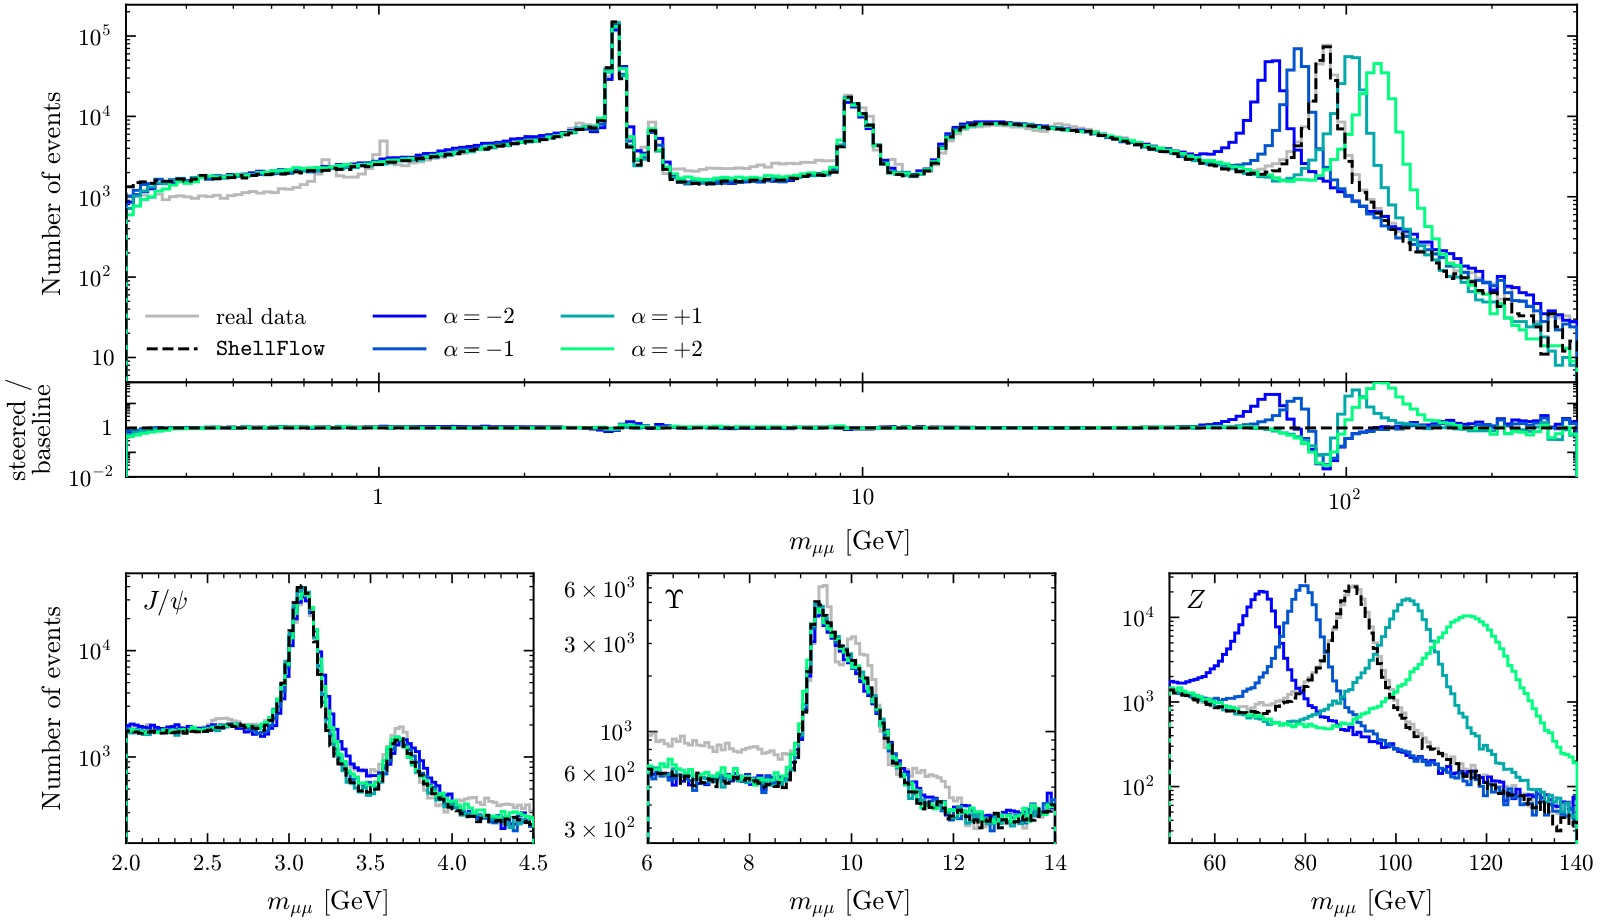
\includegraphics[height=2.45cm]{fig3_spectrum.png}};
\node[fig, anchor=west] (f5) at ($(f3.east)+(0.12,0)$) {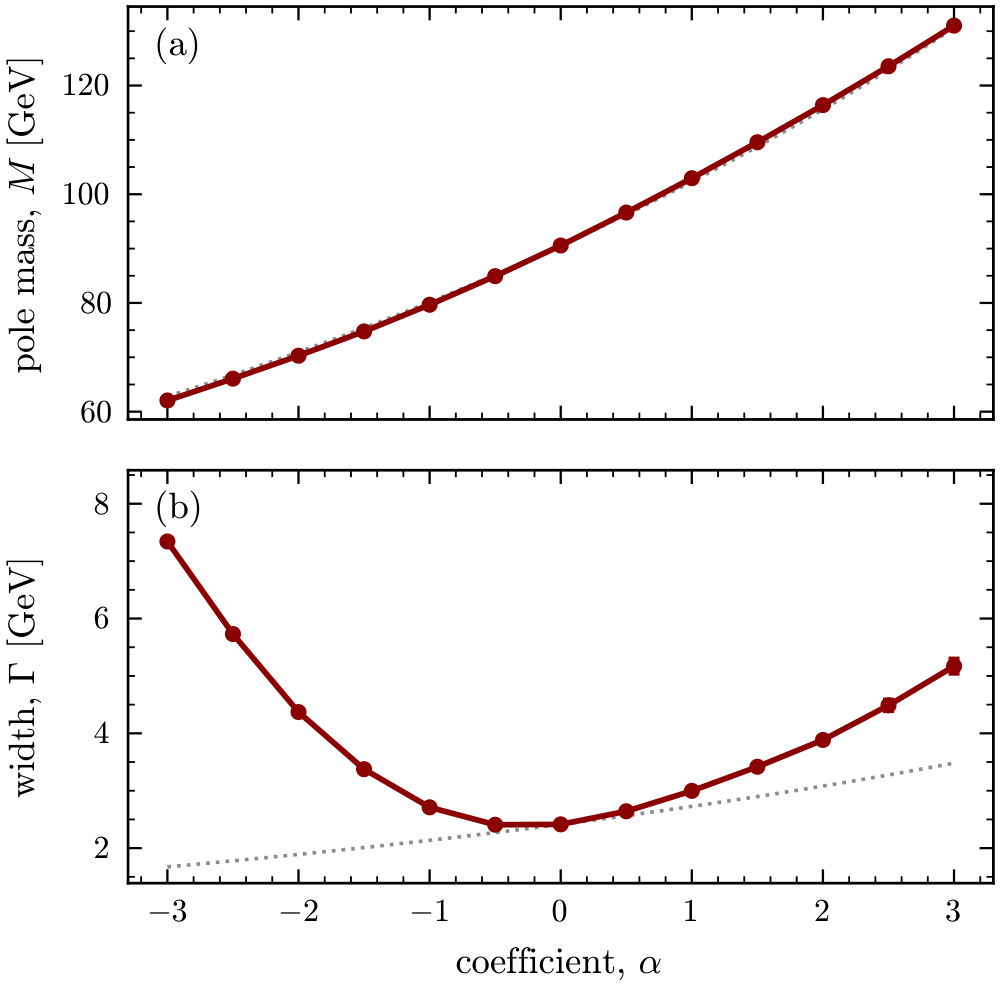
\includegraphics[height=2.45cm]{fig5_pole_width.png}};
\node[figlabel] at (f3.south) {Fig.~3};
\node[figlabel] at (f5.south) {Fig.~5};
\node[fig, anchor=west] (f4) at (\xg,\yc) {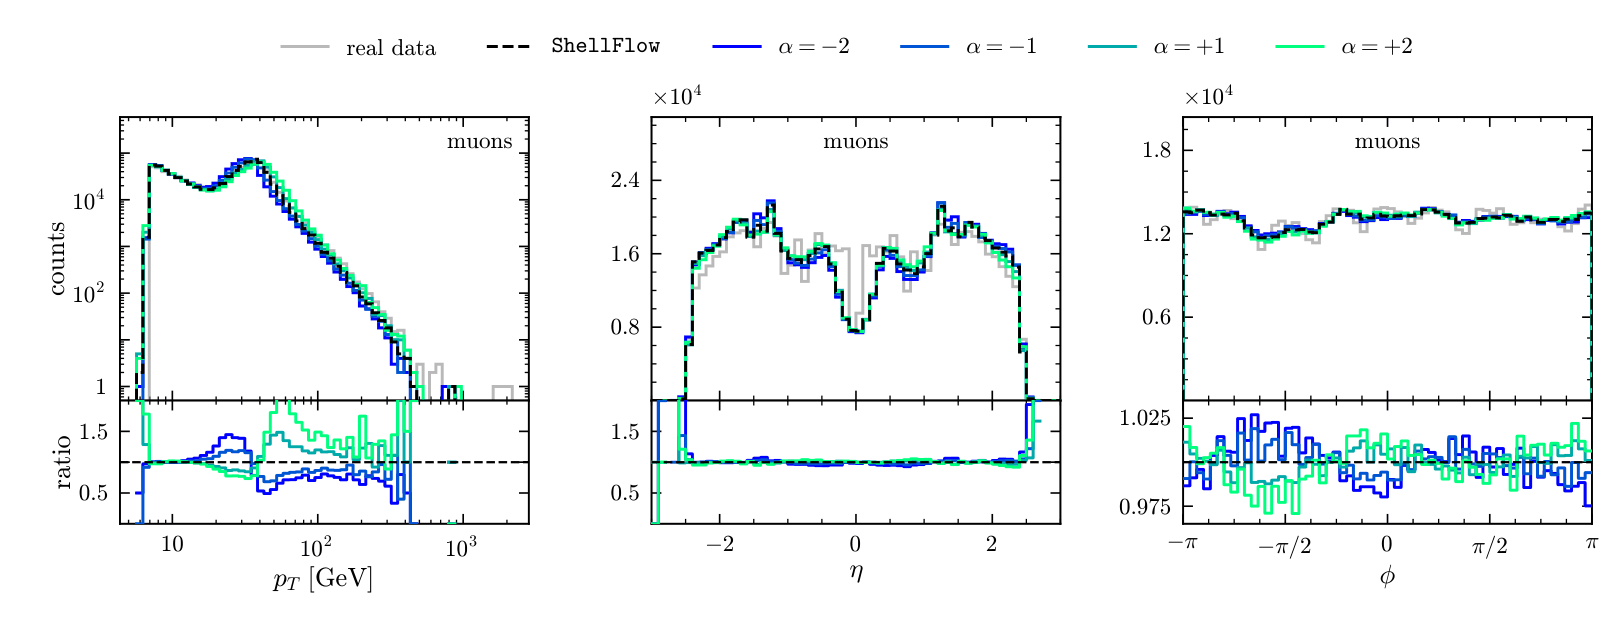
\includegraphics[height=2.45cm]{fig4_kinematics.png}};
\node[figlabel] at (f4.south) {Fig.~4 (and 14)};
\node[fig, anchor=west] (f7) at (\xg,\yb) {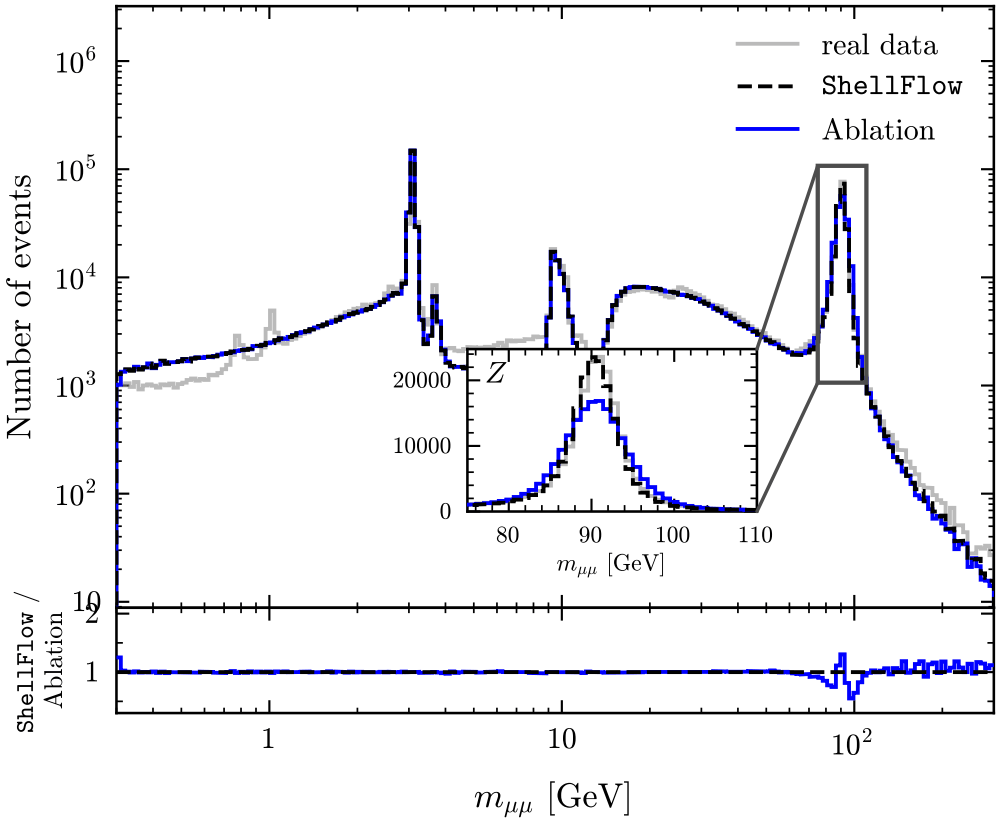
\includegraphics[height=2.45cm]{fig7_ablation.png}};
\node[figlabel] at (f7.south) {Fig.~7};

% ---- chain labels -----------------------------------------------------------------------------------------------
\node[chainlabel] at ($(gen.north west)+(0,0.05)$) {\textcolor{blue!70!black}{steering}};
\node[chainlabel] at ($(kgen.north west)+(0,0.05)$) {\textcolor{green!45!black}{kinematics}};
\node[chainlabel] at ($(am.north west)+(0,0.05)$) {\textcolor{orange!75!black}{mean ablation}};
\node[chainlabel] at ($(grad.north west)+(0,0.05)$) {\textcolor{black!70}{every chain}};

% ---- arrows -----------------------------------------------------------------------------------------------------
\draw[flow] (dir) -- (grad);
\draw[flow] (grad) -- (sv);
\draw[flow] (sv) -- (gen);
\draw[flow] (gen) -- (ro);
\draw[flow] (ro) -- (pl);
\draw[flow] (pl) -- (f3);
\draw[flow] (ste) -- (gen);

\draw[flow] (\trunk,\ya) -- (\trunk,\yc+0.25) -- (kgen.west |- 0,\yc+0.25);
\draw[flow] (\trunk,\yb+0.25) -- (ab.west |- 0,\yb+0.25);
\fill (\trunk,\ya) circle (1.8pt);
\fill (\trunk,\yb+0.25) circle (1.8pt);
\draw[flow] (allfs.east |- 0,\yc-0.25) -- (kgen.west |- 0,\yc-0.25);
% the mean ablation generates the steering sample again, with and without the ablation; the line crosses the arrow
% generate -> readout near its tail, with a white gap that shows the crossing
\def\xcross{\xd+\boxw+0.16}
\draw[white, line width=3pt] (\xcross,\ya+0.25) -- (\xcross,\ya-0.25);
\draw[flow] (ste.east) -- (\xcross,2.75) -- (\xcross,\ya-1.725) -- (\xd,\ya-1.725) -- (ab.north);
\draw[flow] (kgen) -- (kro);
\draw[flow] (kro) -- (kpl);
\draw[flow] (kpl) -- (f4);

\draw[flow] (grad.south) -- (\xb,\yb) -- (am.west);
\draw[flow] (am.east |- 0,\yb-0.25) -- (ab.west |- 0,\yb-0.25);
\draw[flow] (ab) -- (aro);
\draw[flow] (aro) -- (apl);
\draw[flow] (apl) -- (f7);

\draw[shortcut] (ship) -- node[left, font=\fontsize{6.5}{7.5}\ttfamily, align=right, xshift=-2pt, text=accent]
  {steering\_vectors.from\_file\\[-1pt]\textrm{(skips the gradient pass)}} (sv);

\end{tikzpicture}
\end{document}
